
\documentclass[UTF8]{ctexart} 
\usepackage{geometry}                		% See geometry.pdf to learn the layout options. There are lots.
\geometry{a4paper}
%\usepackage[parfill]{parskip}    		% Activate to begin paragraphs with an empty line rather than an indent
\usepackage{graphicx}
\usepackage{amsmath}	
\usepackage{fontspec}
\usepackage{minted}

\graphicspath{ {./images/} }	
	
\title{混沌系统在计算机伪随机数生成中的应用}
\author{信息科学技术学院\\
杨垒\\
1400012791}
\date{\today}							
\begin{document}
\maketitle
\begin{abstract}
随机数在计算机科学中有非常广泛、重要的应用,例如生成网络加密通信中的密钥、用于蒙特卡洛法模拟,等等。用一定的电子计算机算法生成的,满足随机数性质的数字序列称为伪随机数。本文探索使用混沌模型生成伪随机数的可能性,并分析产生的伪随机数序列的性质,最终给出一种新的随机数生成方法。
\end{abstract}

\section{随机数和伪随机数}
一个数字序列如果不含一定的规律或模式,就被称为具有统计学随机性,例如投掷硬币、旋转均匀转盘得到的数列。通过一定测试可以判断一个序列是否具有统计学随机性。例如 M.G. Kendall 和 B. Babington Smith 提出了四个测试\cite{randomnesstest},用于检验序列的统计学随机性。

\begin{description}
  \item[频率测试] 数列中各数字出现的次数是否基本相同。
  \item[序列测试] 数列中各多位数组合出现的次数是否符合随机分布规律。
  \item[扑克测试] 测试数列中每个元素的数字分布情况。例如,元素 101,202,330非常相似,因为它们都有两位相同数字。
  \item[间隔测试] 测试数列中满足一定条件的数之间的间隔。例如,测试一个数列中 0.5 到 1.0 之间的数出现的间隔。
\end{description}

随着理论的发展,现在已经有一系列测试用于判定随机数序列的随机性。本文将采用Linux系统下的ent软件\cite{enttestprogram}分析序列的随机性,并得到4个指标,通过比较实际得出的值和理想随机序列的值确定序列的随机性。

需要注意的是,一个序列拥有统计学随机性并不表明它具有“真随机性”。一个真随机序列还应具有“不可预测性”,即完全无法根据序列的一部分推测出序列的下一个元素。由于真随机序列的产生往往需要从物理现象中获得,例如雷暴产生的电磁波变动、设备所在地辐射场信息等,无法直接通过计算机算法生成,因此本文的讨论范围限制在统计学随机性中。

\section{使用 Logistic 映射产生序列}
\subsection{Logistic 映射}
\subsubsection{定义}
Logistic 映射是一个非线性映射,来自 Robert May 在 1976 年发表的一篇论文\cite{logisticmap}。它的表达式为
\[
x_{n+1}=rx_n(1-x_n)
\]
其中,$x_n$是$[0, 1]$内的数,r是$(0, 4]$内的数。

\subsubsection{性质}
首先求解 Logistic 系统的周期1解。显然,$x=0$是其中之一。
\begin{align*} 
x&=rx(1-x)\\
{1\over r}&={1-x}\\
{x}&={{r-1}\over{r}}
\end{align*}
因此,系统有两个周期1解。

随着参数$r$和启动值$x_0$的不同,Logistic 系统呈现出不同的特性。
\begin{description}
  \item[$0<r<1$] \hfill \\
  \[
  {{x_{n+1}}\over{x_n}}={r(1-x_n)}
  \]
  由于此处$0 <x_n < 1$且$0<r<1$,所以$x_n$会单调递减。最终$x_n$将趋近于周期1解0。
  \item[$1<r<2$] \hfill \\
  $x_n$会单调趋近于周期1解${r-1}\over r$。
  \item[$2<r<3$] \hfill \\
  $x_n$会震荡收敛于周期1解${r-1}\over r$。
  \item[$3<r<3.5699$] \hfill \\
  $x_n$会在多个值之间震荡。
  \item[$3.5699<r\leq4$] \hfill \\
  系统进入混沌状态,对于启动值$x_0$很小的变化,后续也会产生巨大的差异,而且几乎没有周期现象。
  \item[$r>4$] \hfill \\
  系统离开$[0, 1]$区间发散。
\end{description}
\subsection{Logistic 映射的应用}
\subsubsection{参数$r$的确定}
为了使产生的序列具有统计学随机性,序列不应有明显的周期现象。当$r<3.5699$时,序列最终会稳定在一个或数个周期解上,因此这个区间是不可取的。再考虑$r>4$的情形,系统将离开$[0, 1]$区间。事实上,生成随机数序列时,往往需要指定一个区间,故$r>4$的情形也是不可取的。因此,$r$可取的区间落在$(3.5699, 4]$。

当参数$r$处于此区间时,系统进入混沌状态,启动值$x_0$很小的变化会导致后续巨大的差异,因此理论上,稍稍改变$x_0$即可产生完全不同的序列,符合伪随机数的性质。

为了更精确地确定$r$的理想取值,考虑$x_n$可能的分布区间。由重要不等式可得,
\[
x_n(1-x_n)\leq 0.25
\]
即
\[
x_{n+1} \leq 0.25r
\]
即$x_n$在$[0.25r, 1]$内不可能取到值。故$x_n$也无法取到$[0.25r, 1]$区间映射后的区间。显然,要出现混沌现象,$0.25r>0.5$,故由函数的性质,可确定当$x_n\in[0.25r, 1]$时,
\[
0 \leq x_{n+1} \leq 0.25r^2-0.0625r^3
\]
故$x_n$也不可能在$[0, 0.25r^2-0.0625r^3]$区间内取值。事实上,经过多次迭代,可以求出$x_n$的精确取值区间,但它一定是小于$[0, 1]$的。

由以上讨论可知,当参数$r \ne 4$时,$x_n$的取值区间不是$[0, 1]$,而是一个较小的,难以快速确定的区间。理想的随机数生成算法需要一个稳定的取值区间,所以,$r$的理想取值为$r=4$。

\subsubsection{生成 Logistic 映射序列}

为使用Logistic映射生成随机数序列,可编写下列C++程序
\begin{minted}[mathescape,
               linenos,
               numbersep=5pt,
               gobble=2,
               frame=lines,
               framesep=2mm]{cpp}
  #include <iostream>
  using namespace std;
  
  /* 需要生成的随机数数量 */
  #define SEQLEN 100000
  
  /* $x$初始值 */
  #define XINIT 0.9
  
  /* 参数$r$值 */
  #define R 4.0 
  
  /* 迭代计算序列中下一个数 */
  inline double logistic_rand(double r, double x)
  {
      return r * x * (1 - x);
  }
  
  int main()
  {
      volatile double x = XINIT;
      volatile double r = R;
      for (long long i = 0; i < SEQLEN; i++)
      {
          x = logistic_rand(r, x);
          cout << x << endl;
      }
      return 0;
  }
\end{minted}

使用Logistic模型映射计算随机数,只需要执行2次乘法和1次减法,与线性取余法(需要取余等耗时操作)等常用随机数生成算法相比,具有一定的性能优势。为比较Logistic映射和C语言标准函数库中rand()函数的速度,分别用两种方法生成大量随机数,并比较两者消耗的CPU时钟周期数,数据详见表\ref{randomgenerationclock}。

\begin{table}[h]
\centering
\caption{使用不同方法生成大量随机数的耗时}
\label{randomgenerationclock}
\begin{tabular}{ l || c c c c}
数量       & 1M & 10M   & 100M   & 1G      \\ \hline
Logistic & 7304 & 67736 & 656720 & 6473161 \\
rand()   & 9302 & 90023 & 883878 & 9159314 \\
\end{tabular}
\end{table}

\subsection{检验Logistic映射生成序列的随机性}
在使用ent软件精确分析随机性之前,先简单统计生成序列中数的分布状况,所得结果详见表\ref{naivedistribution}

\begin{table}[h]
\centering
\caption{Logistic映射生成序列的数值分布,$r=4.0$,$x_0=0.9$}
\label{naivedistribution}
\begin{tabular}{ l || c c c c c}
区间       & $[0, 0.2)$ & $[0.2, 0.4)$   & $[0.4, 0.6)$  & $[0.6, 0.8)$ & $[0.8, 1.0]$ \\ \hline
100K & 29690 & 14036 & 12902 & 13914 & 29458  \\
1M   & 295078 & 140785 & 128079 & 141008 & 295050 \\
10M & 2952441 & 1407077 & 1280867 & 1408498 & 2951117
\end{tabular}
\end{table}

从结果看,$r=4.0$时Logistic映射生成序列的分布不平均,在边界区分布较多,区间中部较少,且基本呈现对称分布的规律。对不同的$x_0$进行测试可以发现,这一规律对所有启动值$x_0$均适用。

\begin{figure}[h]
\caption{Logistic映射生成序列的分布图,$r=4.0$,$x_0=0.9$}
\centering
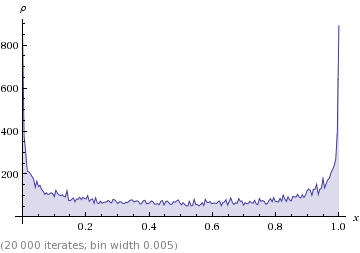
\includegraphics[width=0.75\textwidth]{logdist}
\end{figure}

因此,直接使用$r=4.0$时Logistic映射在$[0, 1]$的生成序列是不可取的。需要对生成算法进行一定的改进。

\section{改进的Logistic随机数生成方法}
\subsection{解决序列分布不均匀}
\subsubsection{帐篷映射}
考虑帐篷映射
\[ x_{n+1}=\begin{cases} 
      \mu x_n & x_n < {1 \over 2} \\
      \mu (1-x_n) & x_n \geq {1 \over 2}
    \end{cases}
\]
当且仅当$\mu = 2$时,这是一个$[0, 1] \to [0, 1]$的映射。事实上\cite{connectiontent},$\mu = 2$时的帐篷映射和$r=4$时的Logistic映射之间只相差一个非线性变换。考虑非线性变换
\[
{y} = {{arccos(1-2x)}\over{\pi}}
\]
容易求得逆变换
\[
{x} = {{1 - cos(\pi y)}\over{2}}
\]
则

\begin{align*} 
{y_{n+1}} &= {{arccos(1-2x_{n+1})}\over{\pi}}\\
&={{arccos(1-8x_n(1-x_n))}\over{\pi}}\\
&={{arccos(cos(2\pi y_n))}\over{\pi}}\\
&=\begin{cases}
  2y_n & y < {1\over2}\\
  2(1-y_n) & y \geq {1\over2}
  \end{cases}
\end{align*}
可知$y_{n+1}=f(y_n)$是$\mu=2$的帐篷映射。而且,由于进行了反三角函数的运算,$y$在计算中有相当大可能性是无理数,在这种情况下,帐篷映射将产生混沌现象。

\subsubsection{生成映射序列}
考虑$\{x\}$经非线性变换得到的序列$\{y\}$,它满足帐篷映射的性质,而且也具有混沌特性。编写如下C++程序生成映射序列$\{y\}$

\begin{minted}[mathescape,
               linenos,
               numbersep=5pt,
               gobble=2,
               frame=lines,
               framesep=2mm]{cpp}
  #include <iostream>
  #include <cmath>
  using namespace std;
  #define PI 3.14159265
  
  /* 需要生成的随机数数量 */
  #define SEQLEN 100000
  
  /* $x$初始值 */
  #define XINIT 0.9
  
  /* 参数$r$值 */
  #define R 4.0 
  
  /* 迭代计算序列中下一个数 */
  inline double logistic_rand(double r, double x)
  {
      return r * x * (1 - x);
  }
  
  int main()
  {
      volatile double x = XINIT;
      volatile double r = R;
      volatile double y;
      for (long long i = 0; i < SEQLEN; i++)
      {
          x = logistic_rand(r, x);
          y = acos(1 - 2 * x) / PI;
          cout << y << endl;
      }
      return 0;
  }
\end{minted}

\subsubsection{检测生成序列的随机性}
与分析Logistic序列随机性的方法类似,先简单统计落在各区间的数的数量,观察其分布是否均匀。使用计算机生成大量生成序列,数据详见表\ref{improveddistribution}。

\begin{table}[h]
\centering
\caption{改进的生成序列的数值分布,$r=4.0$,$x_0=0.9$}
\label{improveddistribution}
\begin{tabular}{ l || c c c c c}
区间       & $[0, 0.2)$ & $[0.2, 0.4)$   & $[0.4, 0.6)$  & $[0.6, 0.8)$ & $[0.8, 1.0]$ \\ \hline
100K & 19955 & 20031 & 20031 & 19951 & 20032  \\
1M   & 200348 & 200110 & 200109 & 199323 & 200110 \\
10M & 2000631 & 2000185 & 2000184 & 1998815 & 2000185
\end{tabular}
\end{table}
可见使用该方法生成的序列分布均匀性很好,很有可能是实用的随机序列。下面使用ent软件进一步检测其随机性。由于ent软件接收二进制流,且以字节为单位计算随机程度,因此在输出之前将原随机序列做$[0, 1] \to [0, 255]$的映射,并向下取整,放入长为1字节的unsigned char类型中并以二进制形式输出,通过UNIX管道输入ent软件中计算。ent软件计算单位字节的信息熵、卡方分布、蒙特卡洛法求得的$\pi$值、算数平均值,以及序列相关系数。表\ref{results}是详细的测试结果。
\begin{table}[h]
\centering
\caption{ent程序测试结果,$r=4.0$,$x_0=0.9$}
\label{results}
\begin{tabular}{ l || c c c c c}
项目       & 单位字节信息熵 & 卡方分布   & 蒙特卡洛法求$\pi$值  & 算数平均值 & 序列相关系数\\ \hline
实际值 & 7.999815 & 256.86 & 3.1137484 & 127.4277 & 0.000591  \\
理想值 & 8 & 256 & 3.1415926 & 127.5 & 0 \\
偏差 & $-0.0023\%$ & $0.33\%$ & $-0.89\%$ & $-0.0567\%$ & ---
\end{tabular}
\end{table}
可见,改进后的随机数生成方法达到了很好的效果,可以用于实际应用。

本文中探索的新随机数生成方法与目前常用的线性取余法等方法相比,最大的优点在于没有长度限制,即没有周期性。这也是利用混沌系统生成随机数的最大优势。传统随机数生成方法由于有周期现象,故只能生成有限长度的随机数序列。而本文中探索的新方法则没有此限制,而且生成的随机数质量高,是较为实用的一种随机数生成方法。


\begin{thebibliography}{9}

\bibitem{randomnesstest}
  M.G. Kendall \and B. Babington Smith,
  \emph{Randomness and Random Sampling Numbers},
  Journal of the Royal Statistical Society 101:1 (1938),
  147-166.
  
 \bibitem{logisticmap}
  May, Robert M, 1976.
  \emph{Simple mathematical models with very complicated dynamics},
  Nature 261(5560):459-467.
  
  \bibitem{enttestprogram}
  John Walker, 2008.
  \emph{Pseudorandom Number Sequence Test Program}, 
  Retrieved from http://www.fourmilab.ch/random/
  
  \bibitem{connectiontent}
  Jeffrey Rauch,
  \emph{Conjugating the Tent and Logistic Maps},
  University of Michigan

\end{thebibliography}
\end{document}  